\chapter{応用例}
\label{chap:ouyou}

本章では、ハイパー楽譜システムによって実現可能な応用例について述べる。

\newpage

\section{楽器練習}
楽器練習の際は気付いたこと・習ったことなどをメモしながら楽譜を使うのが一般的である。
しかし楽譜上でメモ可能な領域は限られており、自由に書くことはできない。
また楽譜は曲単位で独立しているのでメモした情報が各楽譜に散逸してしまったり、そもそもどこに書いたか分からなくなってしまう問題もある。
本システムではレイアウトの制約を受けず自在にメモを書いたり、技術要素毎にページ(図\ref{seja})を用意して情報を一元管理することができる。

\begin{figure}[H]
\centering
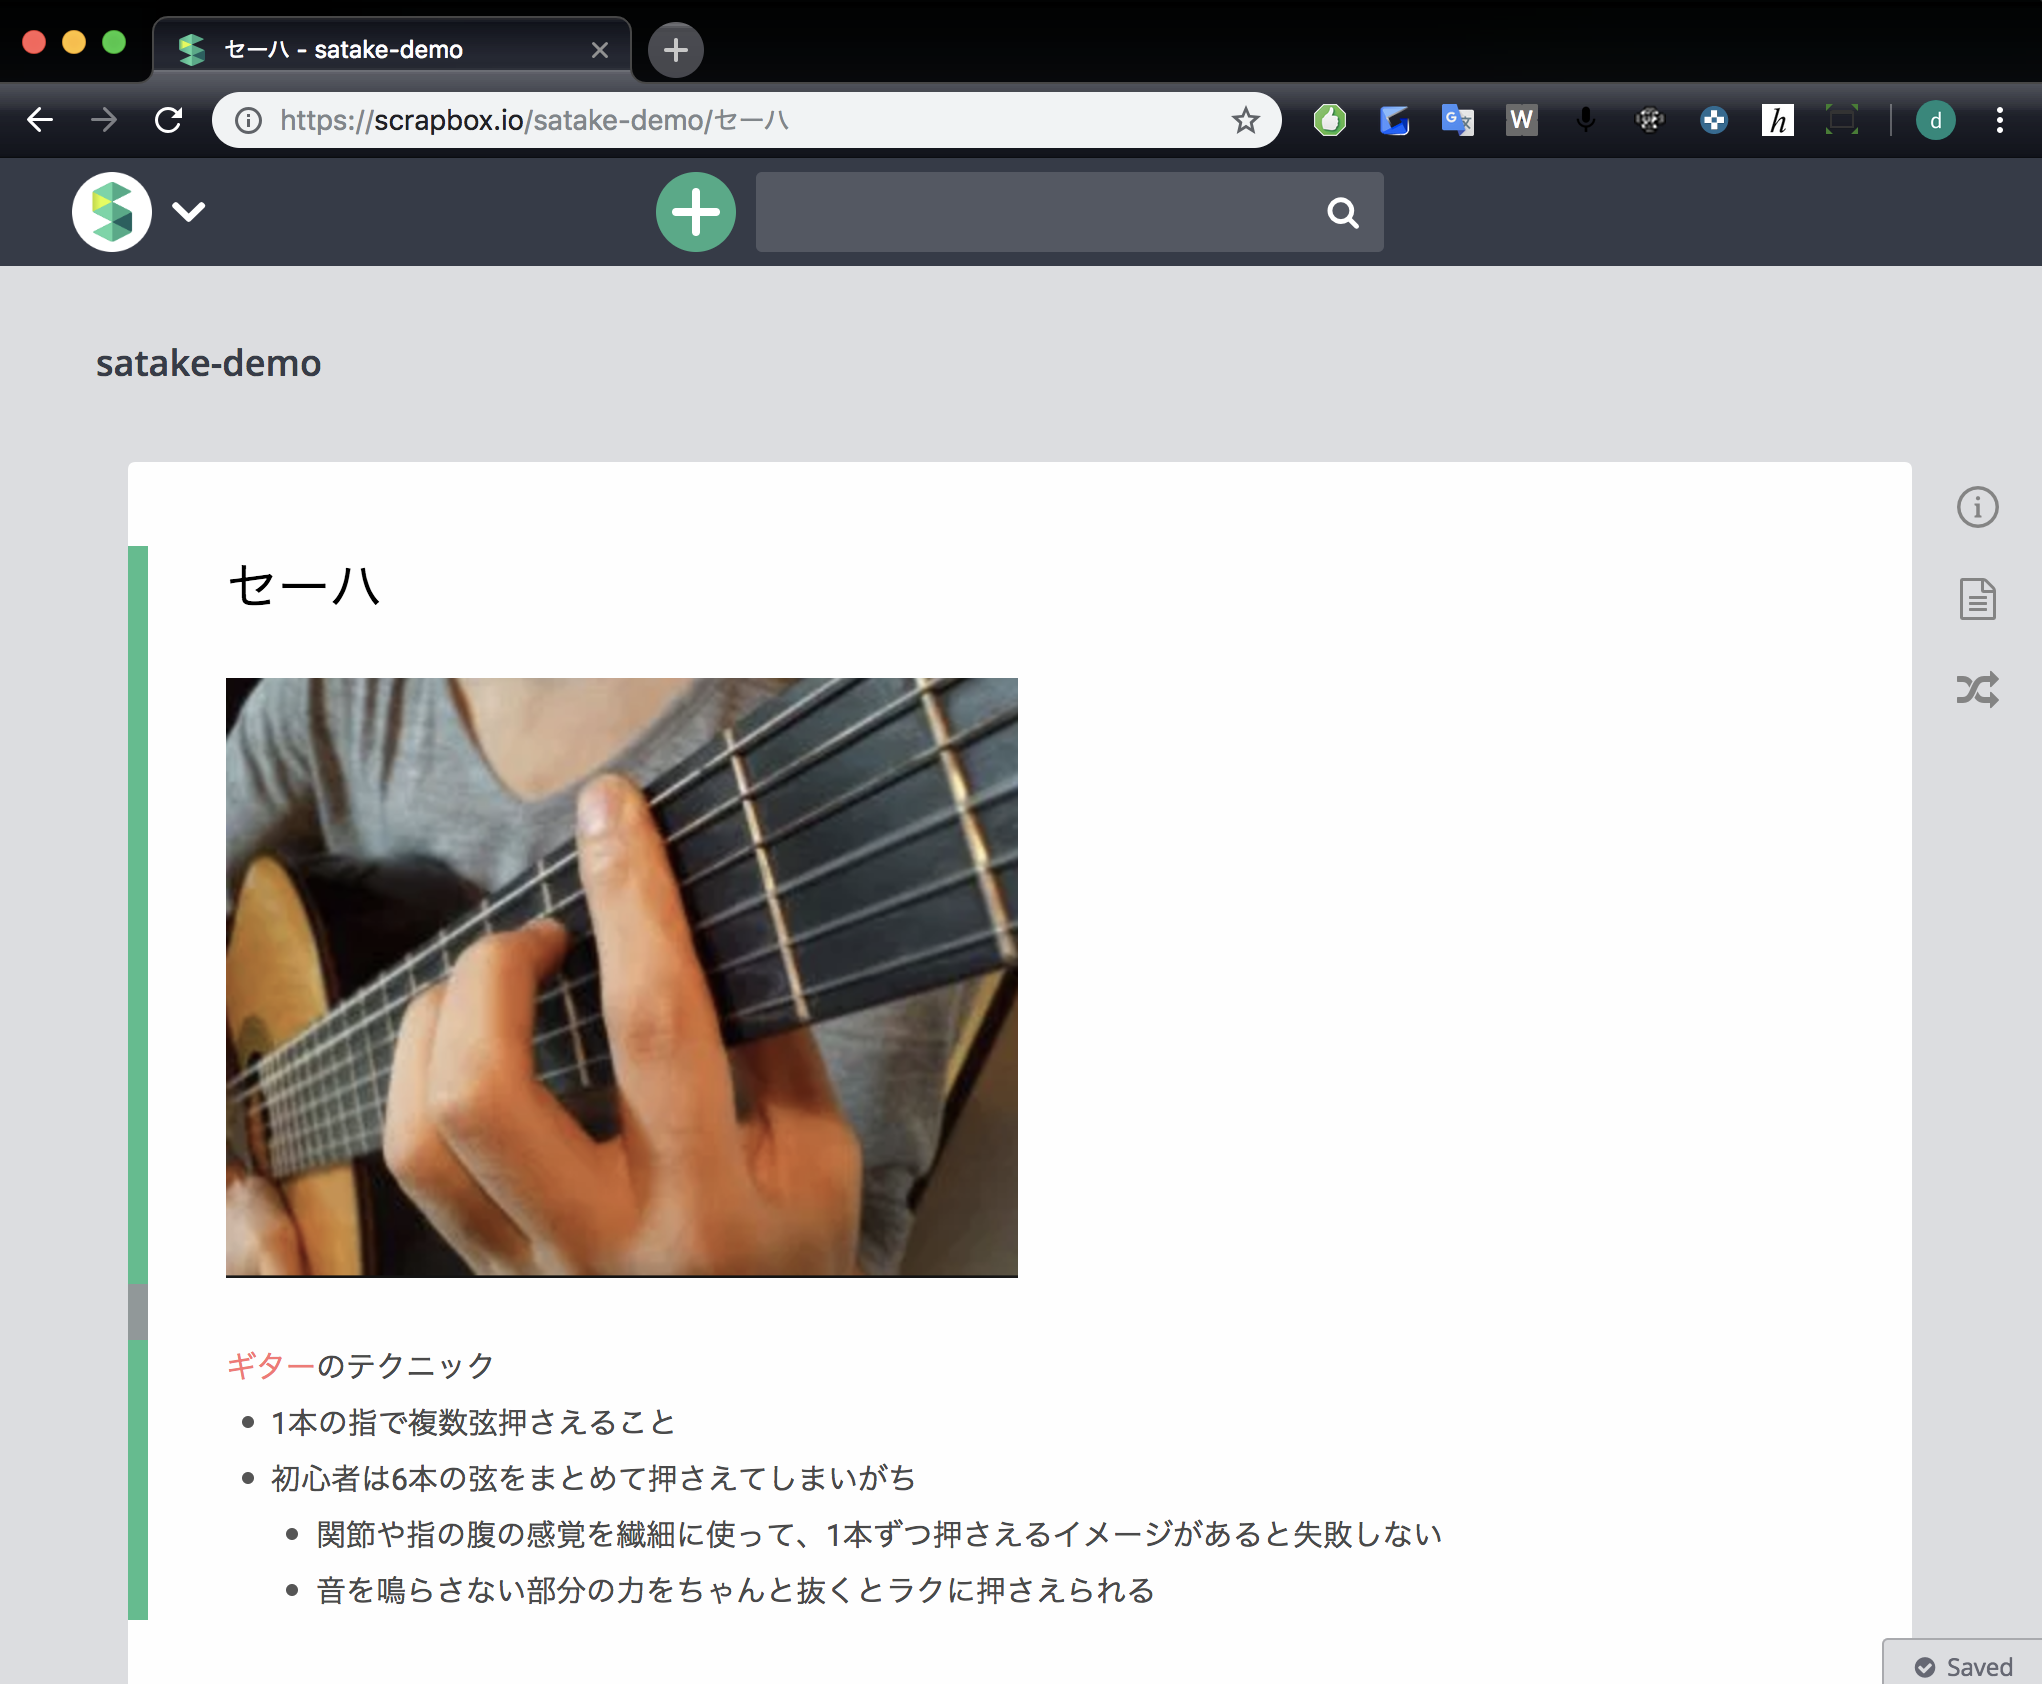
\includegraphics[width=10cm]{images/seja.png}
\caption{技術ページの例}
\label{seja}
\end{figure}

\section{勉強}
楽典や音楽理論といった知識は専門書のように楽譜とは独立した場所に書かれることが多く、学習者が関心のある楽曲との関連性を把握するのが難しい。
本システムでは、楽典や音楽理論といった知識を楽譜と同じScrapboxプロジェクトに記録しておく(図\ref{dominant})ことで、実際の楽曲と結びついた勉強環境を実現できる。
それぞれのページでは楽譜/テキスト/マルチメディアを用いて分かりやすく記述できるだけでなく、ハイパーリンクによって楽曲との関連性を可視化し、勉強/演奏をシームレスに繋げることができる。
そしてページが追加されるうちにたくさんの知識や楽曲がハイパーリンクで結びつき、Scrapboxプロジェクト全体が自分専用の教材として利用できるようになる。
本システムによって、楽譜とテキストのみで表現力が乏しい/実際の楽曲との関連が分からないといった既存の教材の問題点を解決しながら、勉強するだけで教材が作られていくという新しい勉強法を実現できる。

\begin{figure}[H]
\centering
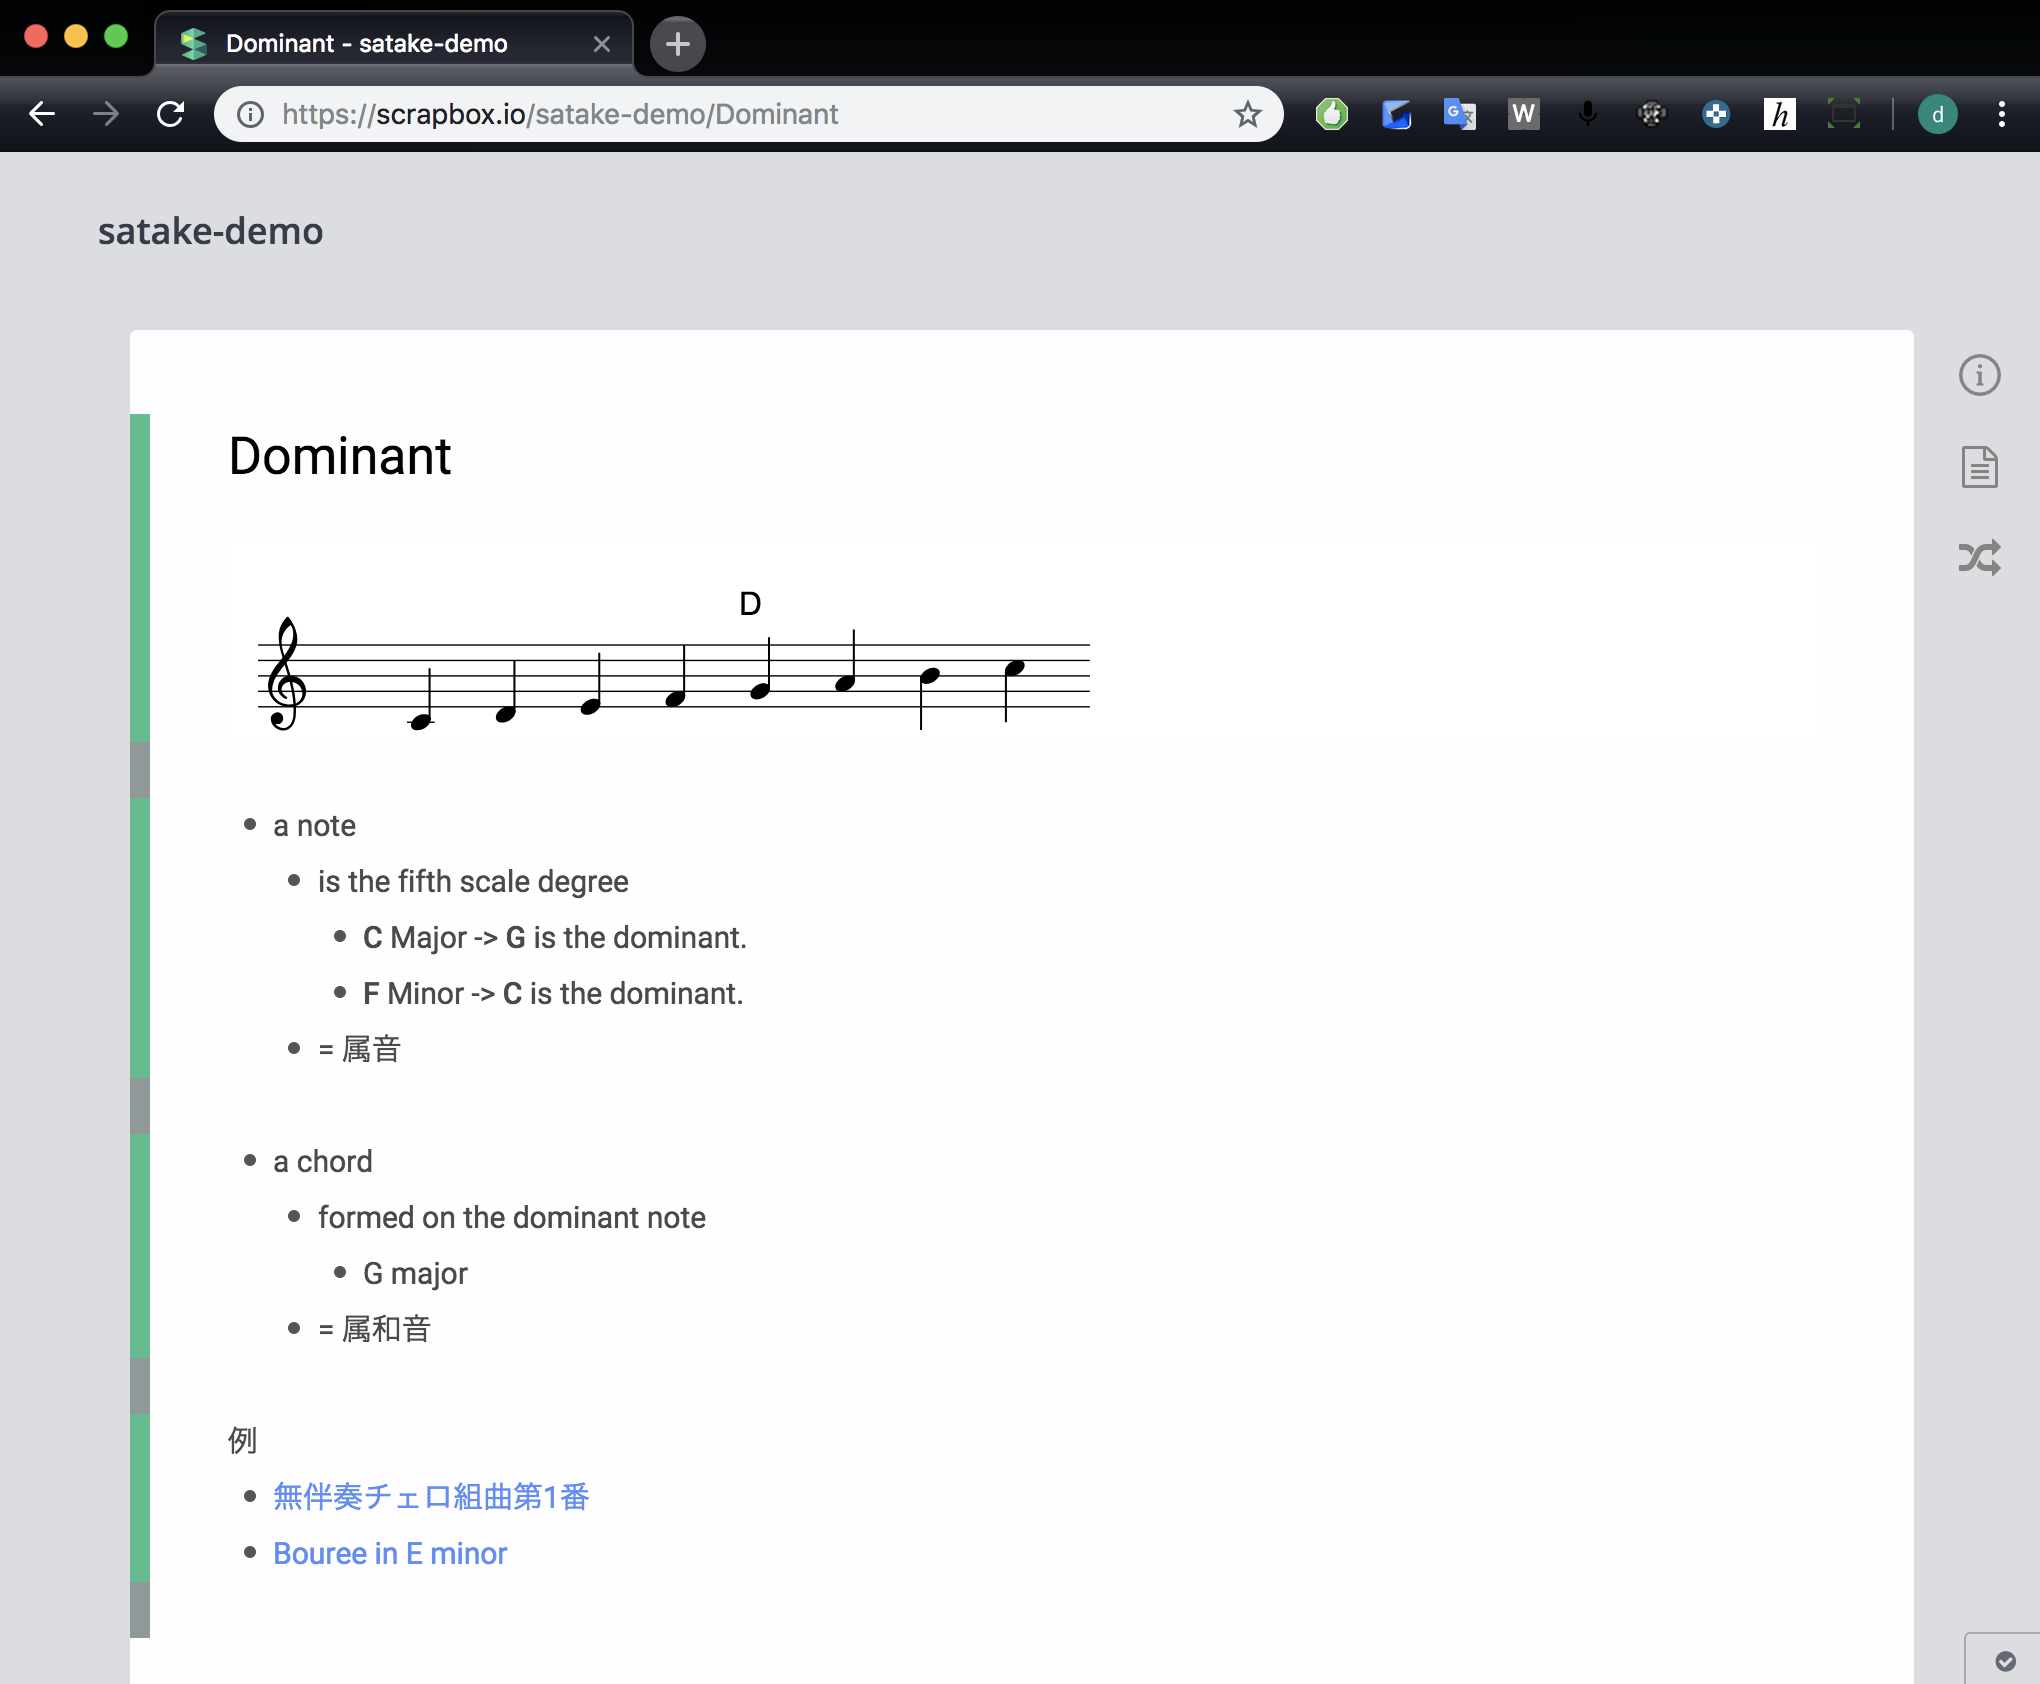
\includegraphics[width=10cm]{images/dominant.png}
\caption{知識ページの例}
\label{dominant}
\end{figure}

\section{楽譜共同編集}
本システムでは楽譜をテキストとして記述しているため、Scrapboxの強力な共同編集機能を活用し、柔軟な楽譜編集を実現できる。
例えば採譜(耳コピ)のような作業をパートや楽章毎に分担することで、大規模な楽譜でも一人一人の負担を軽減することができる。
作曲/編曲といった用途では、作者と演奏者が同じページ上で作業することで、楽譜の変更や演奏者のフィードバックを瞬時に共有することができる。

\section{楽曲の調査/分析}
筆者が所属する増井研究室ではあらゆる情報共有にScrapboxが利用されており、その中には研究に関する話題だけでなく、アニメや音楽といった趣味の情報も多く書かれている。
ハイパー楽譜システムの運用時に、あるアニメ主題歌のメロディやコード進行がとても独創的であったために研究室内で話題になり、Scrapbox上で情報収集や分析が行われるようになった。
その楽曲のページにはYouTube動画や音楽家による考察、作曲者自身のツイートなどがまとめられると同時に、ハイパー楽譜システムを活用して採譜が行われた(図\ref{aobuta})。
音やリズムが適切かというような議論を活発に行いながら楽譜が編集され、楽曲に対する理解が深まったと同時に、和気あいあいと議論しながら曲を分析するという音楽の楽しみ方を発見できた。

もしハイパー楽譜システムが存在しなければ採譜自体が行われなかったと考えられる。
Scrapbox上で楽譜を利用するには楽譜を画像化する必要があり変更が難しくなってしまうし、既存の楽譜作成システムは美しいレイアウトで清書するための環境なので、楽譜を試行錯誤しながら書いたり、断片的にメモ書きするような用途には適さない。

\begin{figure}[H]
\centering
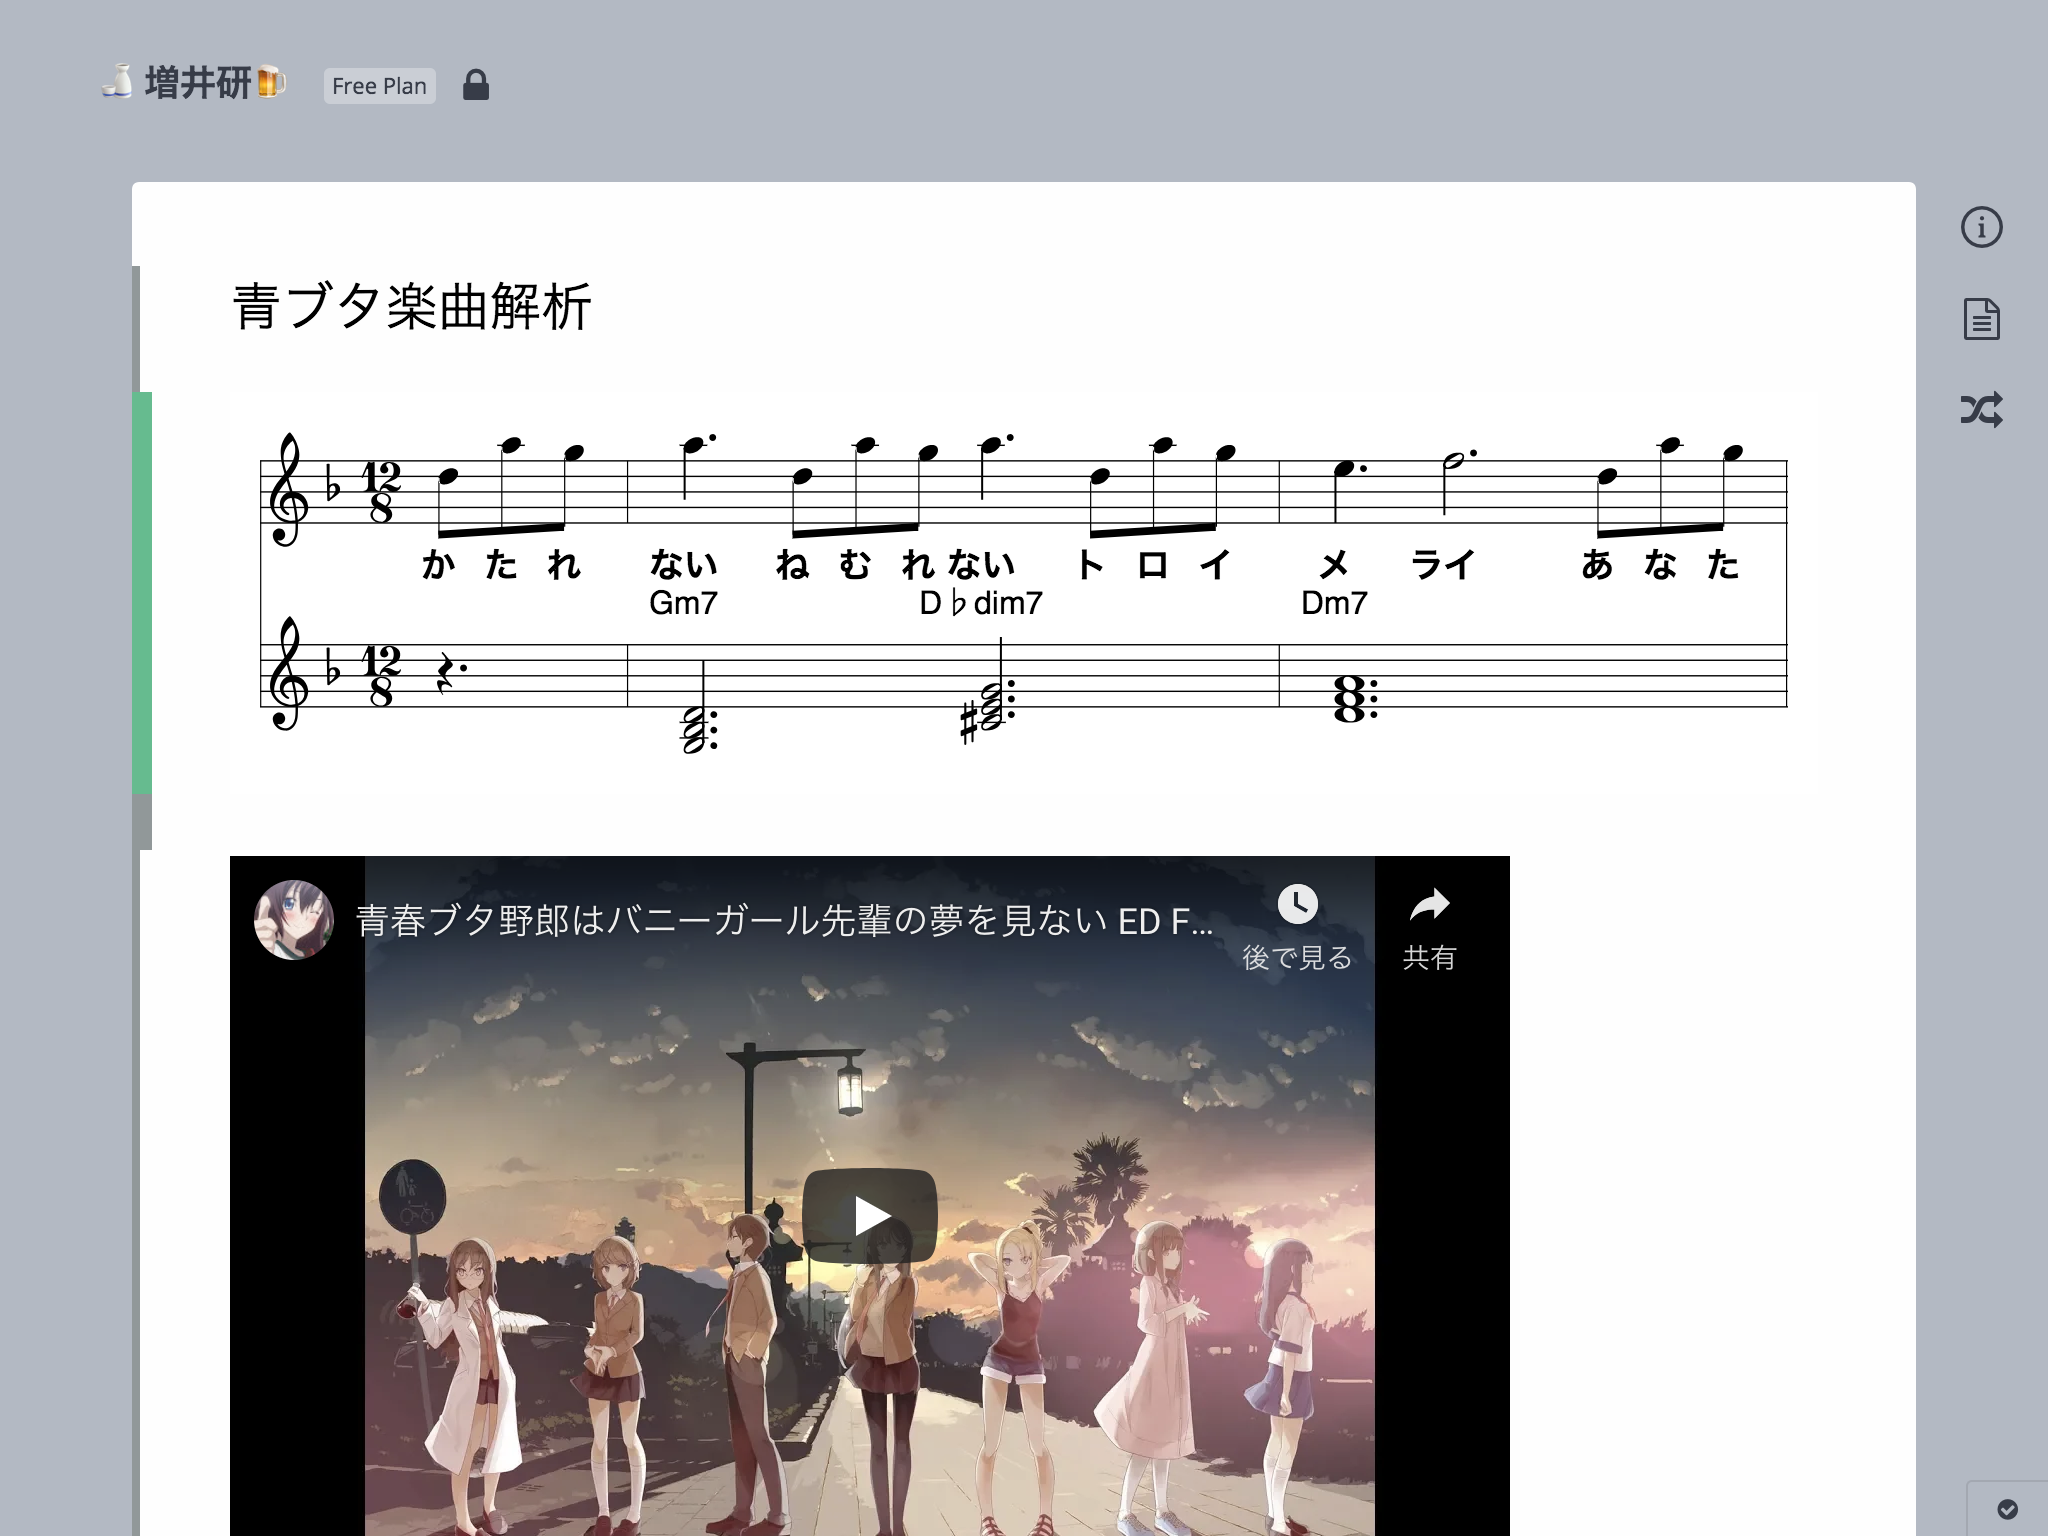
\includegraphics[width=10cm]{images/aobuta.png}
\caption{楽曲ページ}
\label{aobuta}
\end{figure}

\section{まとめ}
本章では、本システムによって実現可能な応用例について述べた。
Wikiと楽譜記述言語の組み合わせによって、今までにない新しい楽譜利用環境の実現が可能である。
本章で述べた応用例に限らず、様々な応用が可能と考えられる。